\documentclass[a4paper,twoside,master.tex]{subfiles}
\begin{document}
\lecture{45}{Friday, December 06, 2019}{Hybrid Orbitals}

\section{Hybrid Orbitals}
\label{sec:hybrid_orbitals}

This morning, we learned about the Coulomb degeneracy and discovered that
\begin{equation}
    E_{kl} = \frac{-E_I}{(k+l)^2}
\end{equation}
Due to this dependency, we replaced the set of quantum numbers $ \{k,l,m\} $ with $ \{n,l,m\} $ where $ n = k + l \geq 1 $, and $ l = 0,1,\cdots,n-1 $. In Hydrogen, this means
\begin{equation}
    E_{2S} = E_{2P}
\end{equation}
Because these states are degenerate, the eigenstates of the Hamiltonian can be linear combinations of these states. This turns out to be critical for bonding models. For example,
\begin{equation}
    \varphi_{n,1,\pm1} = \mp \sqrt{\frac{3}{8 \pi}} R_{n1}(r) \sin(\theta) e^{\pm \imath \varphi}
\end{equation}
\begin{equation}
    \varphi_{n10} \sqrt{\frac{3}{4 \pi}} R_{n1}(r) \cos(\theta)
\end{equation}
We can make linear combinations
\begin{equation}
    \varphi_{nP_x} = - \frac{1}{\sqrt{2}} \left[ \varphi_{n,1,+1} - \varphi_{n,1,-1} \right] = \sqrt{\frac{3}{4 \pi}} R_{n1}(r) \frac{x}{r}
\end{equation}
\begin{equation}
    \varphi_{nP_y} = \frac{\imath}{\sqrt{2}} \left[ \varphi_{n,1,+1} + \varphi_{n,1,-1} \right] = \sqrt{\frac{3}{4 \pi}} R_{n1}(r) \frac{y}{r}
\end{equation}
and
\begin{equation}
    \varphi_{nP_z} = \sqrt{\frac{3}{4 \pi}} R_{n1}(r) \frac{z}{r}
\end{equation}

\begin{figure}[h]
    \centering
    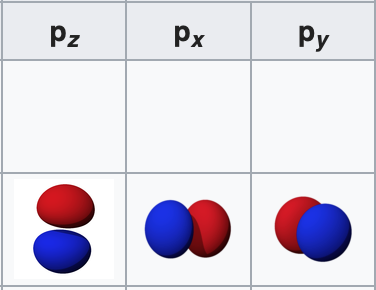
\includegraphics[width=\textwidth/2]{figures/lec_45_pxpypz.png}
    \caption{Plots of the wave functions $ \varphi_{nP_{x/y/z}} $}
    \label{fig:pxpypz_plots}
\end{figure}

Suppose we constructed a linear combination of the $ \varphi_{P_z} $ and $ \varphi_{S} $ wave functions. We call the resulting functions ``hybrid orbitals''.

\begin{figure}[h]
    \centering
    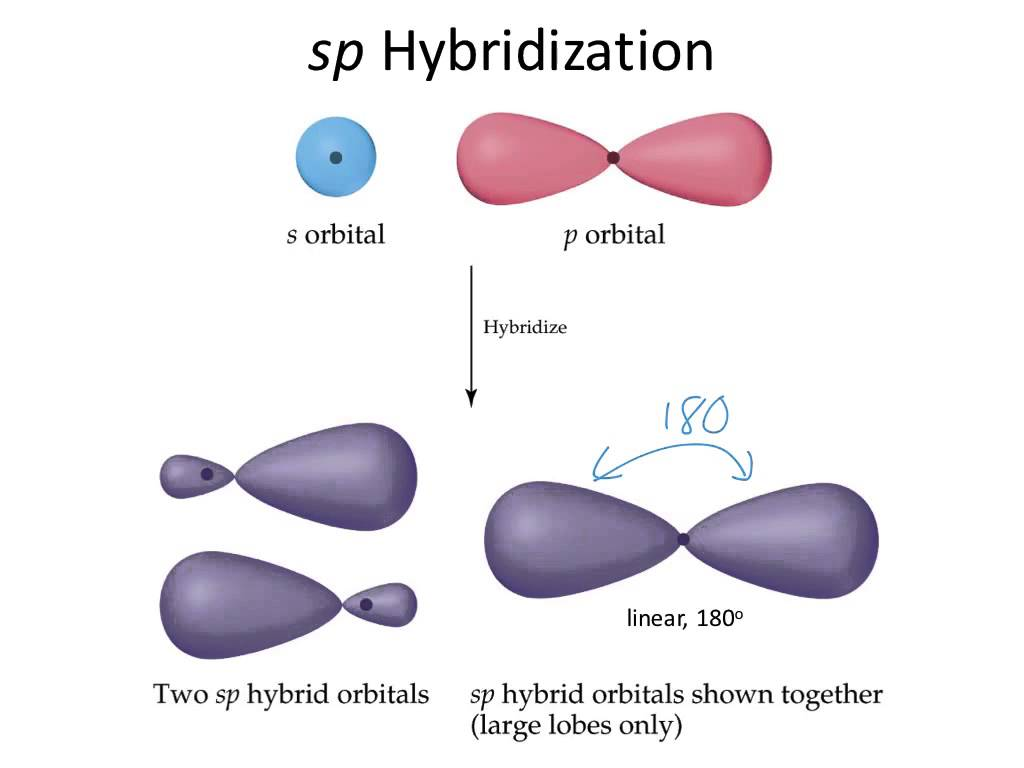
\includegraphics[width=\textwidth/2]{figures/lec_45_sp_hybrid.jpg}
    \caption{$ sp $ hybrid orbitals}
    \label{fig:sp_hybrid_orbitals}
\end{figure}

We can use these hybrid orbitals to understand interatomic bonding in real atoms and real molecules.

\begin{ex}
    Acetylene ($ C_2 H_2 $)
    
    The carbon atoms will have the following electron configuration: $ [1s^2]2s2p^3 $ where the innermost electron is tightly bound and does not interact. On the other hand, hydrogen has the configuration $ 1s $. If we call $ \varphi_{\pm} = \varphi_{P_z} \pm \varphi_{S} $, then we see that the overlapping wave functions between the carbon atoms is an $ s $-like bond which we call a $ \sigma $ bond. Similar bonds will exist between the carbon and hydrogen atoms. Each of these bonds will contain one spin-up and one spin-down electron. Additionally, the $ P_x $ and $ P_y $ orbitals from the carbon atoms can hybridize in planes to form $ \Pi_x $ and $ \Pi_y $ orbitals, which are $ p $-like orbitals since rotation around the $ z $-axis will result in a change in the sign of the wave function.

    In conclusion, the $ C-H $ bonds are single bonds, whereas the bonds between the carbon atoms are triple bonds ($ C \equiv C $), made up of two $ \Pi $ bonds and a $ \sigma $ bond.

\end{ex}

\begin{figure}[h]
    \centering
    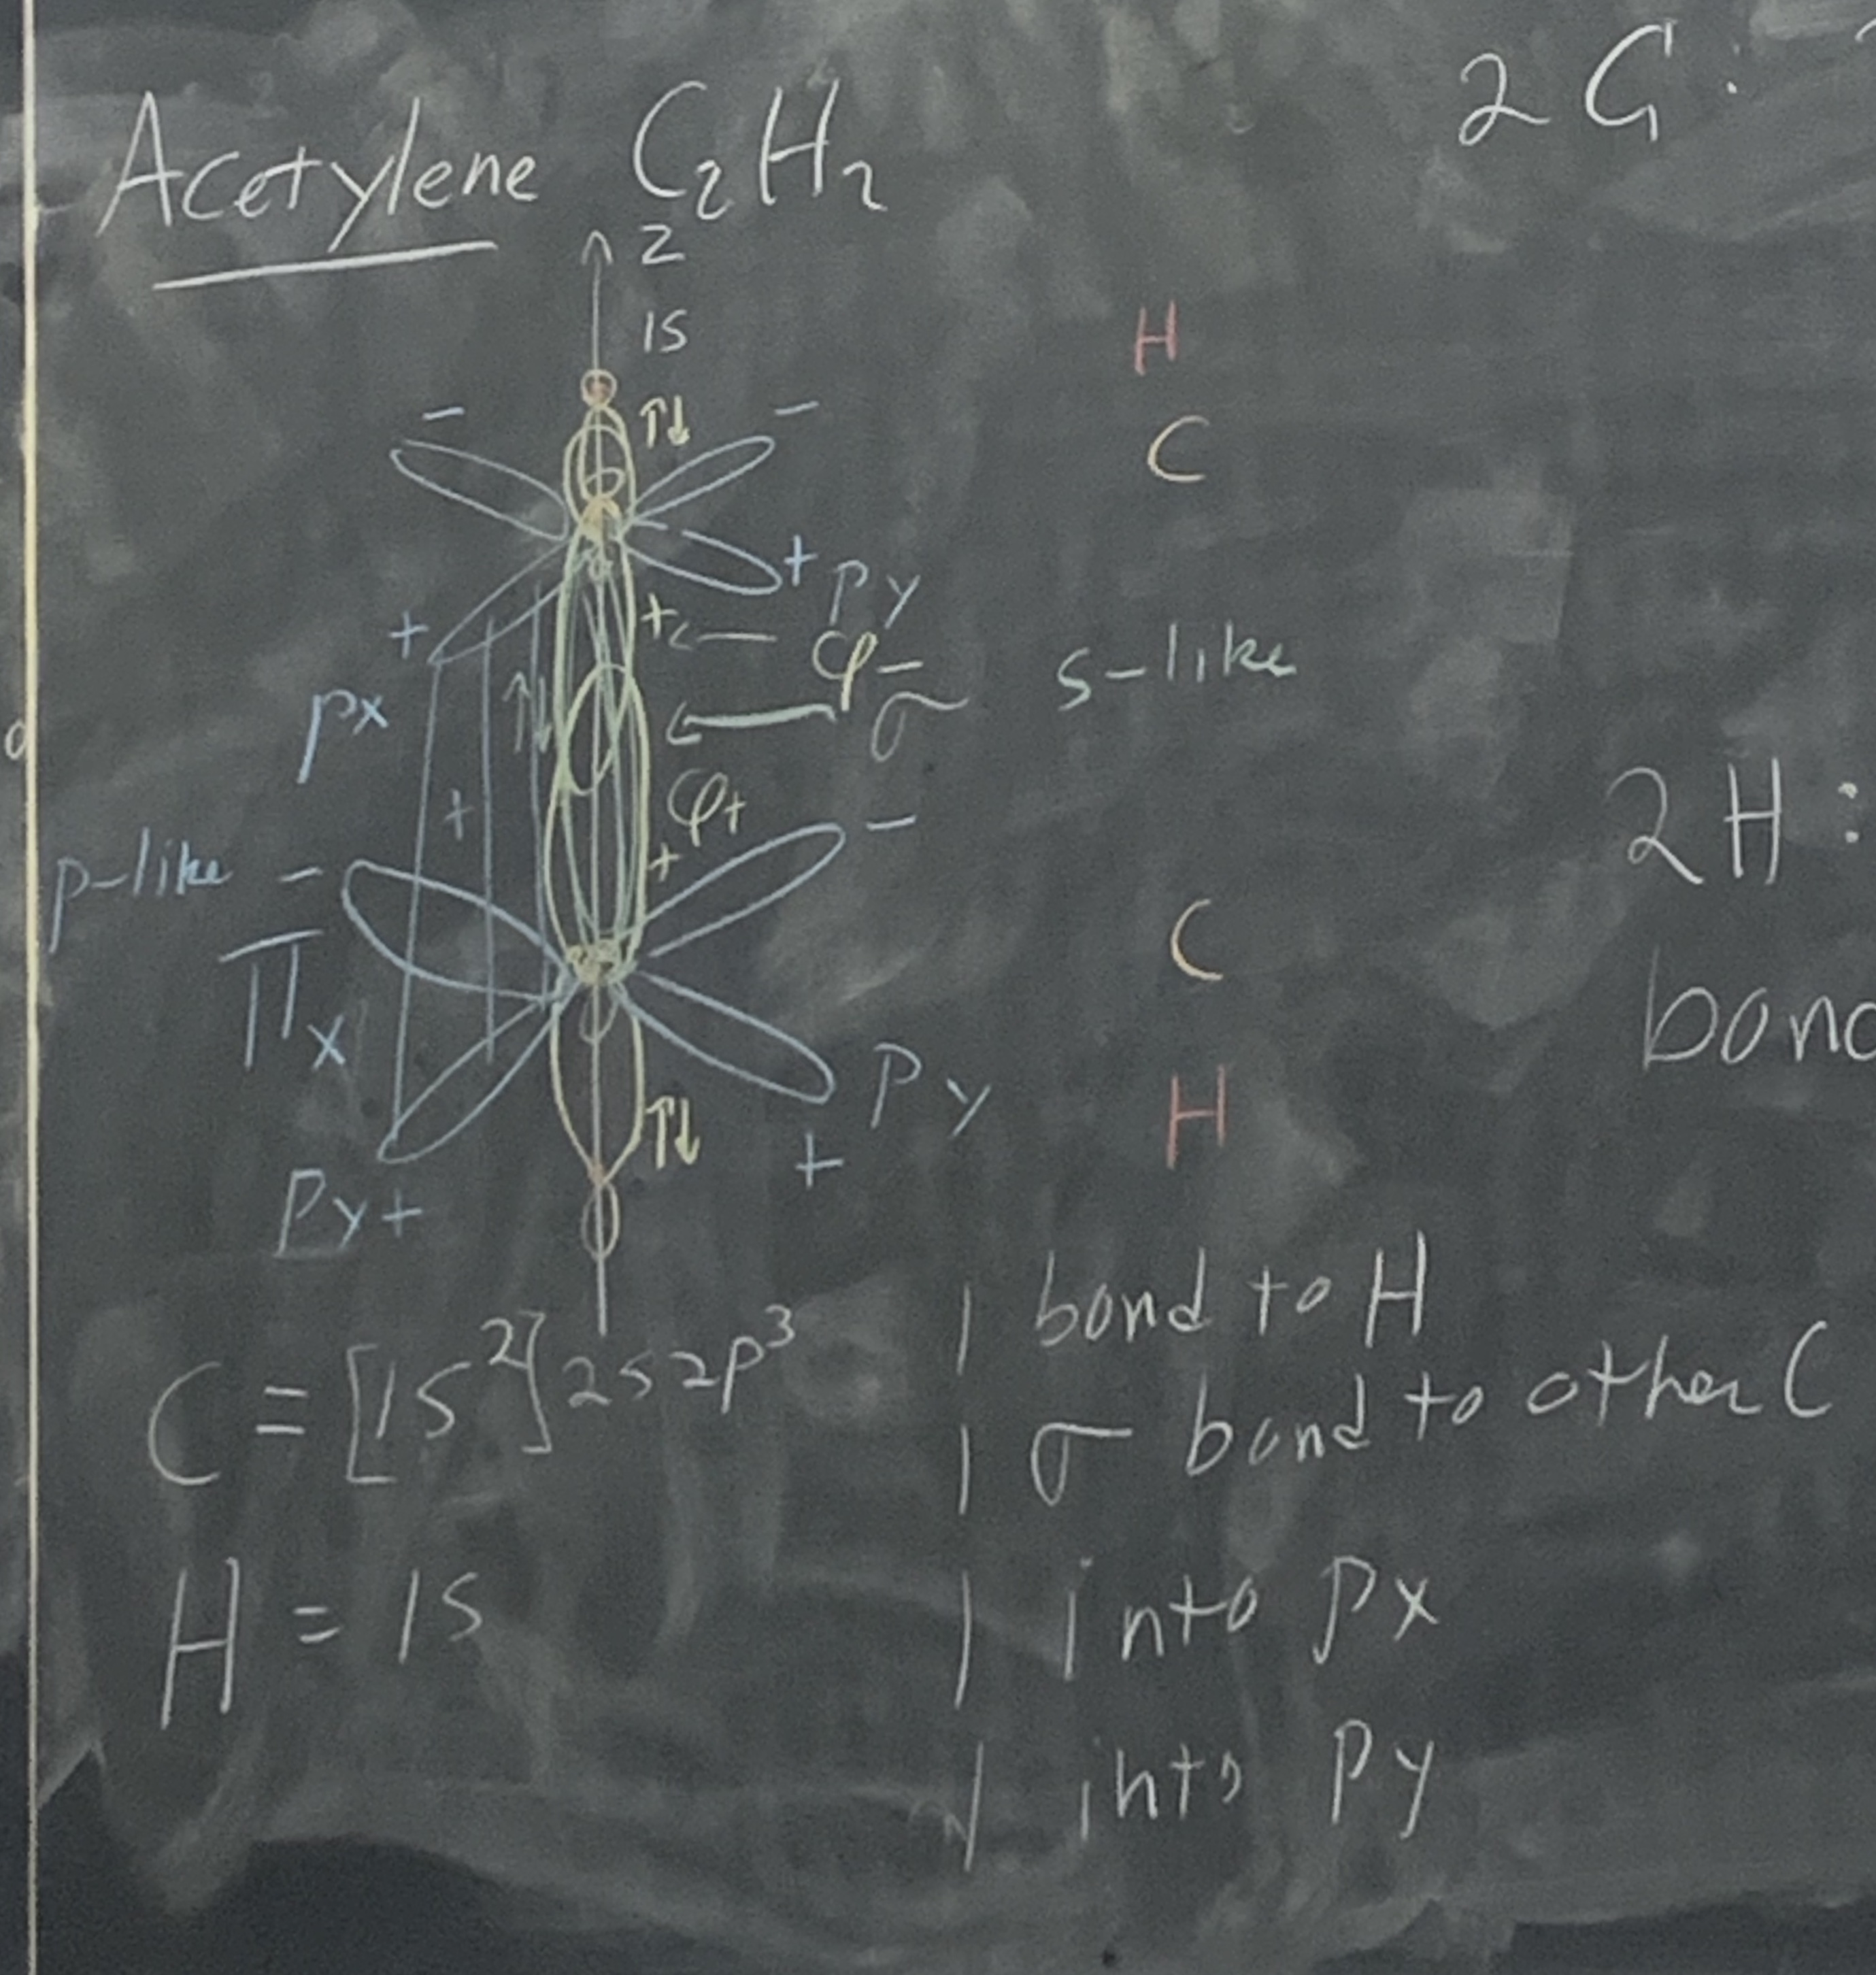
\includegraphics[width=\textwidth/2]{figures/lec_45_acetylene.jpg}
    \caption{The bonding structure of Acetylene}
    \label{fig:acetylene_bonds}
\end{figure}

The $ sp^2 $-hybrids can be described by the wave functions
\begin{equation}
    \varphi_{SP_xP_y} = \frac{1}{\sqrt{3}} \varphi_S + \sqrt{\frac{2}{3}} \varphi_{P_x}
\end{equation}
\begin{equation}
    \varphi''_{SP_xP_y} = \frac{1}{\sqrt{3}} \varphi_S + \frac{1}{\sqrt{6}} \varphi_{P_x} + \frac{1}{\sqrt{2}} \varphi_{P_y} 
\end{equation}
\begin{equation}
    \varphi'''_{SP_xP_y} = \frac{1}{\sqrt{3}} \varphi_S + \frac{1}{\sqrt{6}} \varphi_{P_x} - \frac{1}{\sqrt{2}} \varphi_{P_y} 
\end{equation}

\begin{figure}[h]
    \centering
    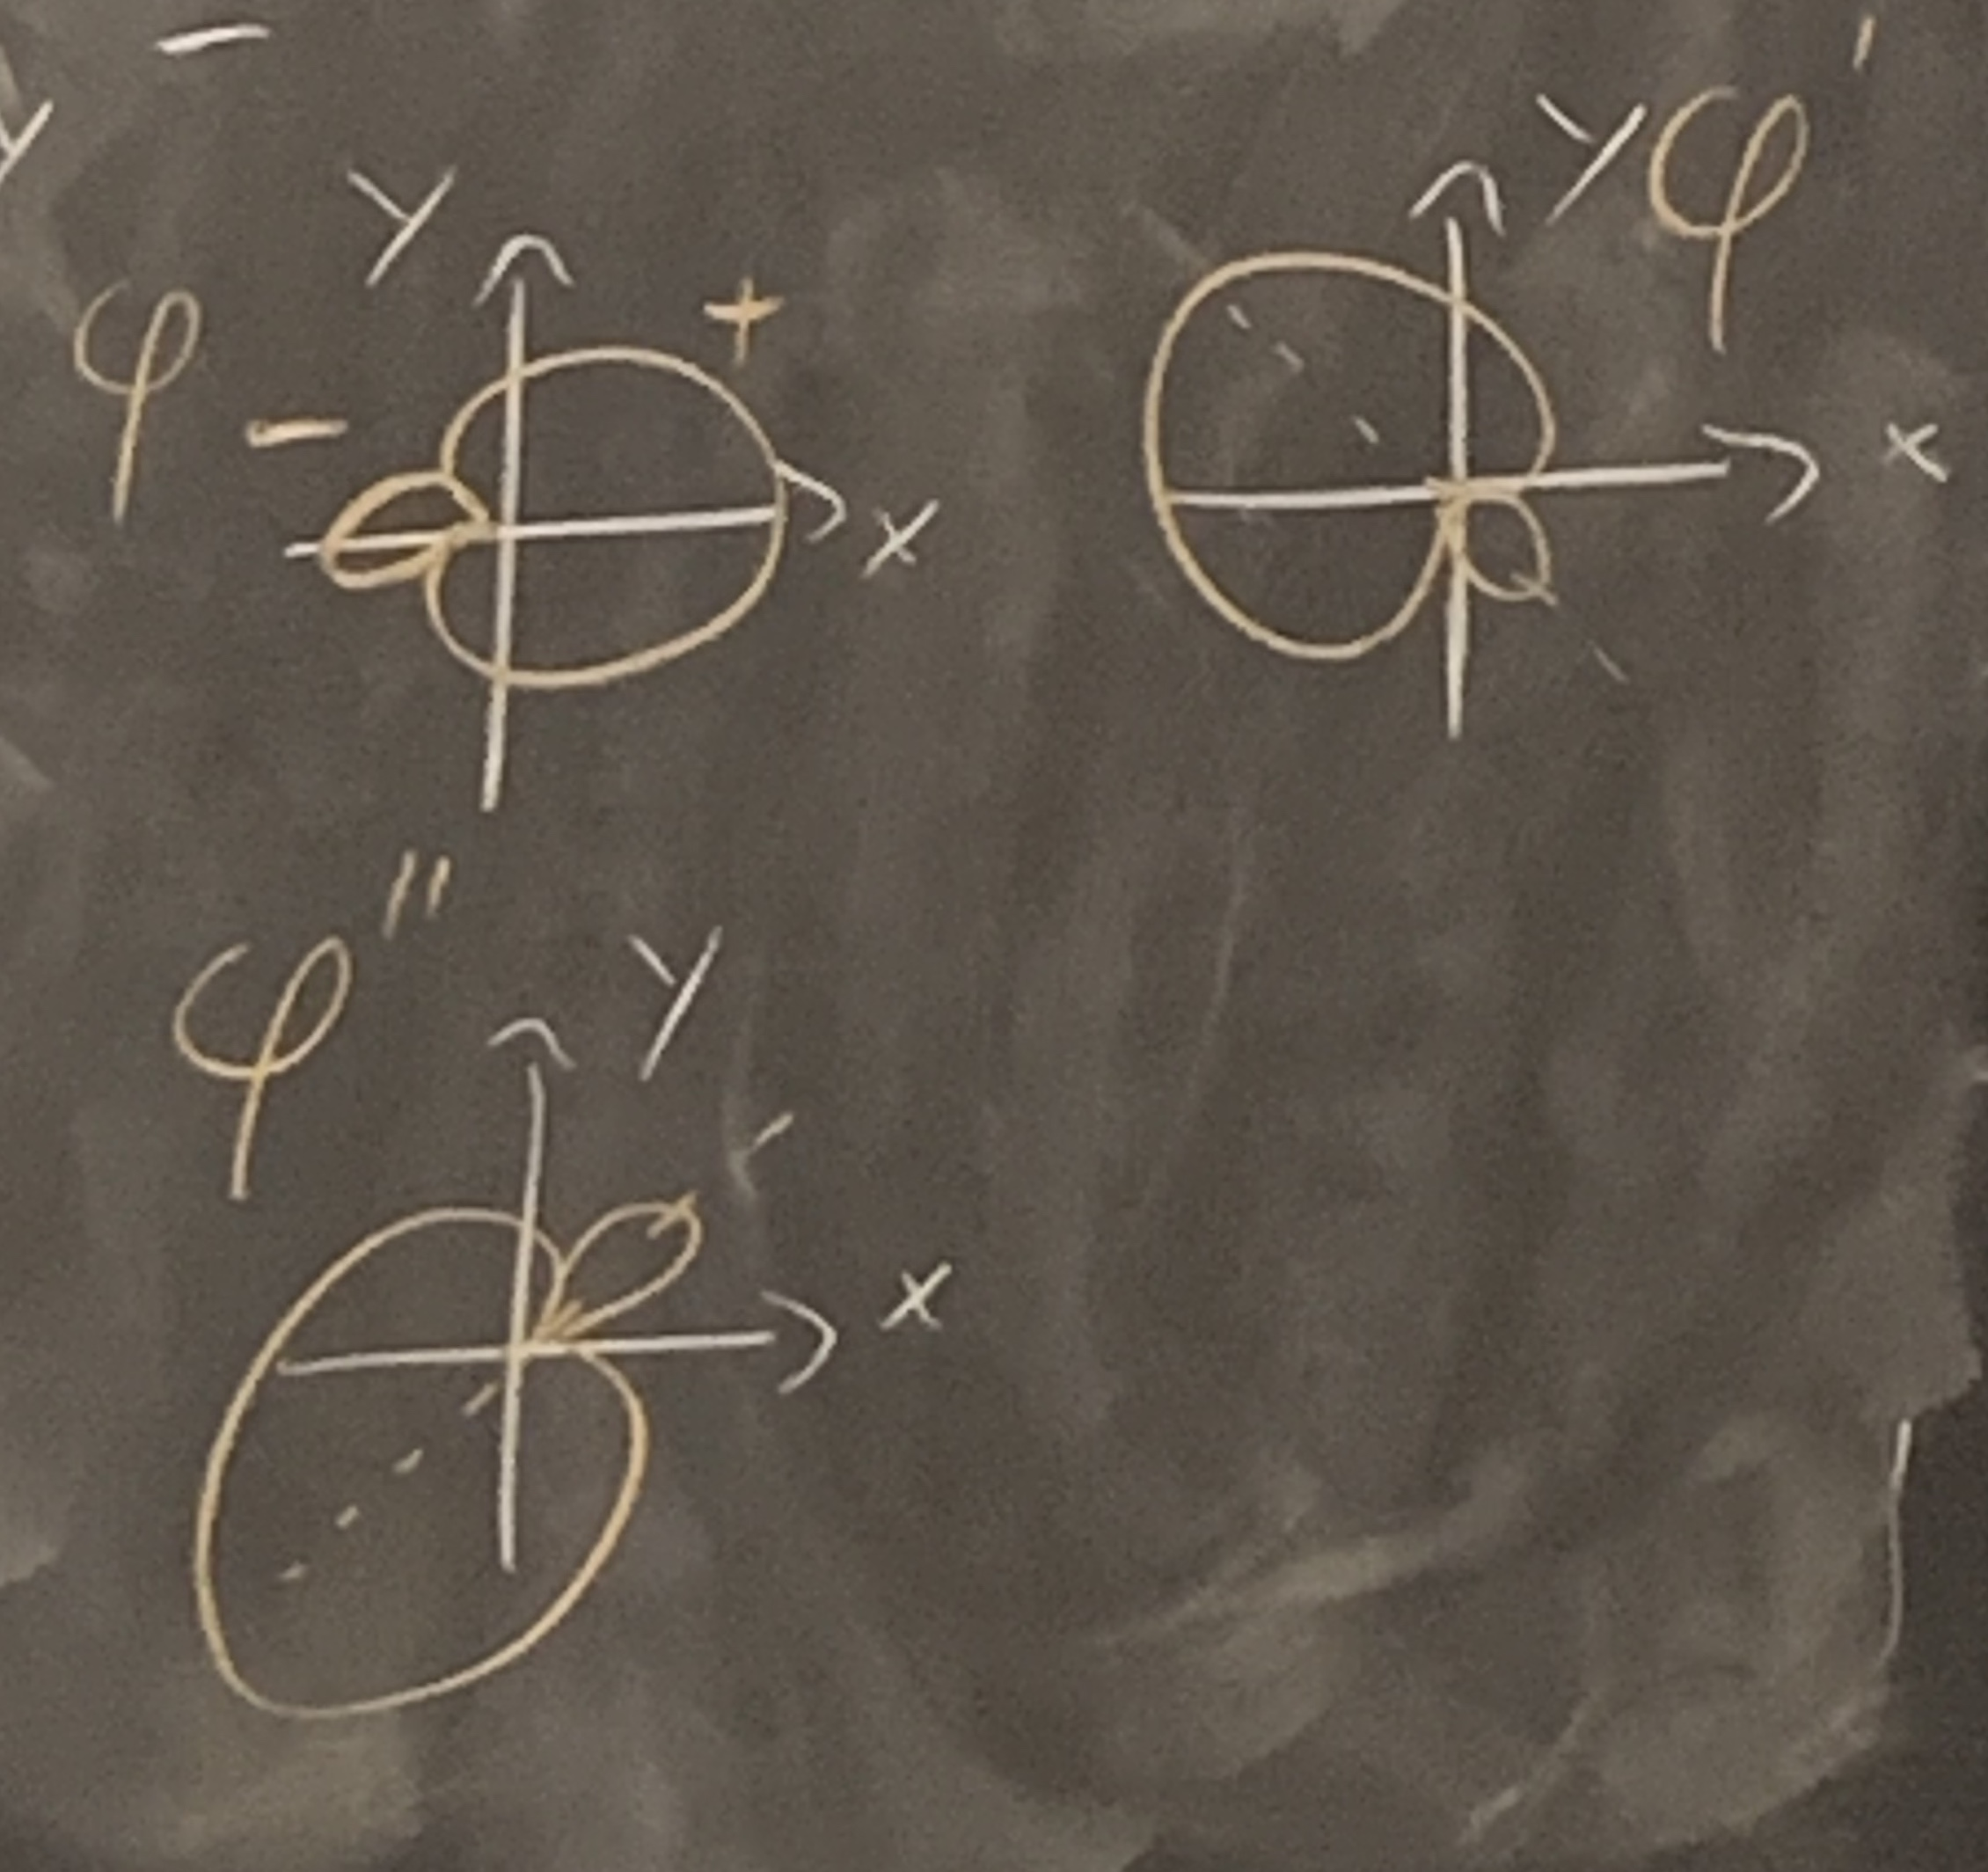
\includegraphics[width=\textwidth/2]{figures/lec_45_sp2.jpg}
    \caption{The $ SP^2 $ Hybrids}
    \label{fig:sp2_hybrids}
\end{figure}

\begin{ex}
    Ethylene ($ C_2 H_4 $) has $ SP^2 $ hybrid orbitals which bond to the hydrogen atoms (the primed orbitals) and to each other (the unprimed orbital). There will also be a $ P_z $ orbital which can bond in a $ \Pi $ bond, creating the double bond between the carbon atoms.
\end{ex}


\end{document}
